\documentclass[draft,final]{thesisclass} % Remove option 'final' to obtain debug information.

% Load packages to allow in- and output of non-ASCII characters.
\usepackage{lmodern}        % Use an extension of the original Computer Modern font to minimize the use of bitmapped letters.
\usepackage[T1]{fontenc}    % Determines font encoding of the output. Font packages have to be included before this line.
\usepackage[utf8]{inputenc} % Determines encoding of the input. All input files have to use UTF8 encoding.

% Extended LaTeX functionality is enables by including packages with \usepackage{...}.
\usepackage{amsmath}    % Extended typesetting of mathematical expression.
\usepackage{amssymb}    % Provides a multitude of mathematical symbols.
\usepackage{mathtools}  % Further extensions of mathematical typesetting.
\usepackage{microtype}  % Small-scale typographic enhancements.
\usepackage[inline]{enumitem} % User control over the layout of lists (itemize, enumerate, description).
\usepackage{multirow}   % Allows table elements to span several rows.
\usepackage{booktabs}   % Improves the typesetting of tables.
\usepackage{subcaption} % Allows the use of subfigures and enables their referencing.
\usepackage[ruled,linesnumbered,algochapter]{algorithm2e} % Enables the writing of pseudo code.
\usepackage[usenames,dvipsnames,table]{xcolor} % Allows the definition and use of colors. This package has to be included before tikz.
\usepackage{nag}       % Issues warnings when best practices in writing LaTeX documents are violated.
\usepackage{todonotes} % Provides tooltip-like todo notes.
\usepackage{hyperref}  % Enables hyperlinking in the electronic document version. This package has to be included second to last.
\usepackage[acronym,toc]{glossaries} % Enables the generation of glossaries and lists of acronyms. This package has to be included last.
\usepackage{lipsum}  % Provides blind text.
\usepackage{acronym} % Provides a list of acronyms.
\usepackage{float} % Provides the H float modifier option.

% Define convenience functions to use the author name and the thesis title in the PDF document properties.
\newcommand{\authorname}{Hannes Brantner} % The author name without titles.
\newcommand{\thesistitle}{Enhancing recruitment efficiency by exploring the impact of large language models on the screening process} % The title of the thesis. The English version should be used, if it exists.

% Set PDF document properties
\hypersetup{
    pdfpagelayout   = TwoPageRight,           % How the document is shown in PDF viewers (optional).
    linkbordercolor = {Melon},                % The color of the borders of boxes around hyperlinks (optional).
    pdfauthor       = {\authorname},          % The author's name in the document properties (optional).
    pdftitle        = {\thesistitle},         % The document's title in the document properties (optional).
    pdfsubject      = {LLMs in HR},              % The document's subject in the document properties (optional).
    pdfkeywords     = {Machine Learning, HR, Human Resources, AI, LLM} % The document's keywords in the document properties (optional).
}

\setpnumwidth{2.5em}        % Avoid overfull hboxes in the table of contents (see memoir manual).
\setsecnumdepth{subsection} % Enumerate subsections.

\nonzeroparskip             % Create space between paragraphs (optional).
\setlength{\parindent}{0pt} % Remove paragraph indentation (optional).

\makeindex      % Use an optional index.
\makeglossaries % Use an optional glossary.
%\glstocfalse   % Remove the glossaries from the table of contents.

% Set persons with 4 arguments:
%  {title before name}{name}{title after name}{gender}
%  where both titles are optional (i.e. can be given as empty brackets {}).
\setauthor{Ing. Dipl.-Ing.}{\authorname}{BSc}{male}
\setadvisor{}{Michaela Wawra}{MSc}{female}

% For bachelor and master theses:
% \setfirstassistant{Pretitle}{Forename Surname}{Posttitle}{male}
% \setsecondassistant{Pretitle}{Forename Surname}{Posttitle}{male}
% \setthirdassistant{Pretitle}{Forename Surname}{Posttitle}{male}

% For dissertations:
% \setfirstreviewer{Pretitle}{Forename Surname}{Posttitle}{male}
% \setsecondreviewer{Pretitle}{Forename Surname}{Posttitle}{male}

% For dissertations at the PhD School and optionally for dissertations:
% \setsecondadvisor{Pretitle}{Forename Surname}{Posttitle}{male} % Comment to remove.

% Required data.
\setregnumber{01614466}
\setdate{01}{10}{2023} % Set date with 3 arguments: {day}{month}{year}.
\settitle{\thesistitle}{\thesistitle} % Sets English and German version of the title (both can be English or German). If your title contains commas, enclose it with additional curvy brackets (i.e., {{your title}}) or define it as a macro as done with \thesistitle.
\setsubtitle{}{} % Sets English and German version of the subtitle (both can be English or German).

% Select the thesis type: bachelor / master / doctor.
% Bachelor:
% \setthesis{bachelor}
%
% Master:
\setthesis{master}
\setmasterdegree{master} % dipl. / rer.nat. / rer.soc.oec. / master
%
% Doctor:
%\setthesis{doctor}
%\setdoctordegree{rer.soc.oec.}% rer.nat. / techn. / rer.soc.oec.

% For bachelor and master:
\setcurriculum{Master in Business Administration (One Year MBA)}{Master in Business Administration (One Year MBA)} % Sets the English and German name of the curriculum.

% Optional reviewer data:
\setfirstreviewerdata{Affiliation, Country}
\setsecondreviewerdata{Affiliation, Country}

% Add glossary entries.
\newglossaryentry{LLM}
{
    name=Large Language Model,
    description={A Large Language Model is reading and emitting text, enabling it to perform tasks such as translation, summarization, and question answering.}
}
\newglossaryentry{TTH}
{
    name=time-to-hire,
    description={The time from the receiving of the candidate's application to the accepted job offer.}
}

\begin{document}

\frontmatter % Switches to roman numbering.
% The structure of the thesis has to conform to the guidelines at
%  https://informatics.tuwien.ac.at/study-services

% \addtitlepage{naustrian} % German title page.
\addtitlepage{english} % English title page.
\addstatementpage

% citation tutorial
% cite only page 1
% \cite[1]{discrimination_algorithms} \newline
% cite page 2 to 5
% \cite[2-5]{discrimination_algorithms} \newline
% cite page 3 and the following page
% \cite[3f]{discrimination_algorithms} \newline
% cite page 3 and the following pages
% \cite[3ff]{discrimination_algorithms} \newline

\begin{acknowledgements*}
\lipsum[1]
\end{acknowledgements*}

\begin{abstract}
\lipsum[1]
\end{abstract}

% Select the language of the thesis, e.g., english or naustrian.
\selectlanguage{english}

% Add a table of contents (toc).
\tableofcontents % Starred version, i.e., \tableofcontents*, removes the self-entry.

% Switch to arabic numbering and start the enumeration of chapters in the table of content.
\mainmatter

\chapter{Introduction}

\section{Background}
\subsection{Large Language Models}
The machine learning model type \gls{LLM} is commonly abbreviated as \acs{LLM} and makes natural language texts processable for computers.
The model works by compressing the read text into an internal state and based on this state an output text is generated.
As the model compresses the data according to the learned patterns in the training data, it does not understand the text in the same way as humans do.
These models are used to perform tasks such as translation, summarization, and question answering \cite[1]{llm_literature_review}.
As this enabled a wide field of automation for application fields that were primarily carried out by humans, many technology companies have developed their own \acs{LLM} and made their services available to the public while keeping their source code mostly private.
Some notable example are the PaLM 2 model by Google \cite{palm2} that powers Bard, the GPT-4 model by OpenAI \cite{gpt4} that powers ChatGPT and the Llama 2 model by Meta \cite{llama2}.
The Llama 2 model is the only model from the picked three candidates that has been released with public source code.
That means that researches and engineers around the world can use the model as building block and either improve the underlying mechanisms or try to incorporate it in their own applications.
The real breakthrough of \acs{LLM}s came with the release of the GPT-3 model by OpenAI \cite{gpt3} that powered the initial version of ChatGPT.
They offered the model's capabilities as a website that was accessible to the public and allowed users to insert text and receive a response from the model.
As described in \cite[1]{gpt3}, the model provided very good performance on various \acs{NLP} datasets that include tasks like translation and question answering.
To briefly visualize the complexity behind a \acs{LLM}, consider the function $f_{a,b,c}(x) = ax^2+bx+c$ that has the three parameters $a$, $b$ and $c$.
Here, the function $f$ maps the input data denoted as $x$ to the output data denoted as $f(x)$.
The input data in the \acs{NLP} case is the input text and the output data is the output text.
\acs{LLM}s also make use of parameterized and differentiable functions in their internal structure to map the input text to the output text, but they have orders of magnitudes more parameters than this sample function.
For example, the model GPT-3 uses 175 billion parameters \cite[1]{gpt3} in total. The parameter count of GPT-4 was not disclosed in their technical report \cite{gpt4}.
The training data needed to train these models was present in the required amounts because the researchers have not used reinforcement learning \cite{rl_bible} or supervised learning \cite[3]{sl_bible}.
Reinforcement learning gives the model a reward when an action was good and a punishment when an action was bad, this can be done by letting the model train in the real world which has bad scalability or in simulators that must be coded to mimic the real world which is also a very difficult and time consuming task.
For example, animals learn that behaviors that lead to food are good and behaviors that lead to hunger are bad.
The supervised learning approach labels input data with the desired output label and based on these mappings and a huge amount of training samples, the model will adjust its parameters to map the input data correctly.
An example would be input images that would be labeled with the object that can be seen on the images. So each input image must be labeled by hand before the model can be trained to predict it itself correctly.
To compress the patterns in the training data and fill them into the model parameters, huge amounts of training data are needed as the parameter count of \acs{LLM}s is huge.
Both techniques were not sufficient to train models of that sheer size, so the researchers used a technique called self-supervised learning \cite[7]{llm_literature_review} where the model tries to fill in artificially generated gaps in the text.
Because the gaps are artificially introduced, the expected output is known in advance, so the model can be trained without the need of labeled training data which makes this technique very scalable.
Before the text is fed to the model it is tokenized \cite[4]{llm_literature_review}, that means the text is converted into a sequence of tokens which can either be symbols, characters, subwords and words.
The model gets the tokenized text input and predicts the follow-up output tokens that will likely follow these input tokens. The output tokens are converted back into text and then the text from the artificial gap is compared to the model output.
Based on this comparison, the model parameters are adjusted. As no human data labelling or costly real-world or simulator training is needed, the model can be trained on huge amounts of data.
Most of the text data used for training large language models is scraped from the internet \cite[1]{llm_literature_review}.
The context size of a \acs{LLM} is the number of tokens that the model can store in its internal state while generating the output tokens, so it is the history of tokens it can access while generating the response.
For example, the context size of the Llama 2 model is 4096 tokens \cite[47]{llama2}.
The tokenizer that OpenAI is using, can be accessed via this website \cite{openai_tokenizer}.
The output tokens of a \acs{LLM} are generated token by token, so when the first token is generated, it is appended to the input and the model generates the next token based on the input that now contains the first generated token. Afterwards, it is run iteratively in the same way.
That means that the total output token size is also constrained by the context size, when the full history of tokens should be within the context size while generating the output.
The model stops the output loop, when the model emits the stop token. That means that it has finished the output token generation.
Most of \acs{LLM}s are based on the machine learning model type called Transformers \cite[1]{transformer} which is a neural network architecture that is based on the attention mechanism.

\clearpage

\section{Problem Statement} \label{problem_statement}
As described in \cite[1]{ai_recruiting}, the average firm's value by 2000 was roughly consisting of 65\% of value from intangible assets.
This has evolved a lot, as by the end of 1980, around 70 to 90\% of tangible assets were accountable for the average firm's value \cite[1]{ai_recruiting}.
This means that the value of a firm is more and more dependent on the quality of its employees and the knowledge they possess and this ongoing process does not seem to come to a halt in the near future.
The technological context of how companies recruit people has also evolved a lot over the last decades, as machine learning tools are more and more used to automate processes or assist humans in attracting the right candidates, screening, assessing and selecting them \cite[2]{ai_recruiting}.
The article \cite[2-4]{ai_recruiting} described four evolution stages of recruiting which are the following:
\begin{enumerate}
    \item \textbf{Analog Recruiting} \label{analog_recruting}\\
    The first stage is the analog recruiting stage where people were the main mechanism of recruiting new employees.
    Prospective applicants needed to go to the company to manually turn a paper job application in.
    Companies want to maximize the information richness they supply for the current job vacancy but also the information reach to attract as many promising applicants as possible.
    But as described in \cite[2]{ai_recruiting}, in analog recruiting these two goals faced the analog reach and richness frontier as shown in \ref{fig:analog_reach_richness_frontier} because the more information is supplied, the more costly it is when you supply to media with great reach at that time:
    \begin{figure}[H]
        \centering
        \includegraphics[scale=0.5,page=2,width=0.6\linewidth,trim={300 100 55 515},clip]{literature/ai_recruiting.pdf}
        \caption{Analog reach and richness frontier \cite[2]{ai_recruiting}}
        \label{fig:analog_reach_richness_frontier}
    \end{figure}
    \item \textbf{Digital Recruiting 1.0} \label{digital_recruiting_1}\\
    This first evolution stage of digital recruiting that happened in the late 1990s was characterized by breaking the analog reach and richness frontier by using digital media which allowed to supply rich information to many prospective candidates at a very low cost because there were no printing and low distribution costs involved.
    There was also a change on the applicant's side as no more manually filled out documents were required to be handed in physically at the company site.
    It also allowed them filter out job offers based on various selectors and it also allowed companies to offer more dynamic content to the job seekers by adding video and audio data to the job search websites.
    There was also a considerable exponential and self-enforcing network effect that was ongoing at that time for job search websites \cite[3]{ai_recruiting}.
    As they listed more and more job offers, more and more job seekers were attracted to the platform which made it easier to persuade companies to list their job offers on the job search websites.
    \item \textbf{Digital Recruiting 2.0} \label{digital_recruiting_2}\\
    This evolution step emerged around ten years after the first evolution of Digital Recruiting and was mainly driven by two developments.
    The first development was the rise of job board aggregation services that presented all job offers from various job search websites on one platform.
    Job seekers now have access to all available job offers without having to visit each platform individually and job firms do not need to publish their offer at each individual website.
    The second development was the introduction and rise of professional social network platforms such as \textit{LinkedIn}.
    These network platforms allowed people to form professional communities and groups of interest and also allowed companies to present themselves to the public and to potential applicants.
    Moreover, with endorsements people in such platforms could endorse skills of others which allowed to build a reputation and trust in the community.
    It enabled companies to target their job ads more effectively to promising candidates, contact candidates directly through the network and also enabled a cheap and efficient way to post job offers on large social websites whether they are professional or not like \textit{Facebook} \cite[3]{ai_recruiting}.
    \item \textbf{Digital Recruiting 3.0} \label{digital_recruiting_3}\\
    After Digital Recruiting matured from 2010 to 2015, Digital Recruiting 3.0 emerged and was primarily driven by the rise of machine learning and artificial intelligence in human resources processes.
    As digital recruiting digitized the processes and also made the processes more frictionless for employers and employees, more and more applications came in for each job offer, on average the number is around 250 applications per job offer \cite[4]{ai_recruiting}. 
    This can be explained by the fact that the cost of applying is very low for the applicant, but this led to about 80\% of the applications being unqualified \cite[4]{ai_recruiting}.
    To deal with this massive amount of applicants, you can either deploy more human resources to screen the applications or you can use machine learning to either automate processes or assist humans such that they can work more productively.
    Human Resources are mission-critical for companies as the human capital is getting more and more important for the success of a company.
    Moreover, research showed that top performers are four to eight times more productive that the average performers, increasingly so in complex environments, according to \cite[4]{ai_recruiting}.
\end{enumerate}
This should have made the need for an effective human resources pipeline clear. To improve this pipeline machine learning tools are deployed to the following four fields \cite[4-8]{ai_recruiting}:
\begin{enumerate}
    \item \textbf{Outreach}\\
    Firms try to identify candidates and get job opportunities in front of them in a way that invites them to
    actually apply. Machine learning can help to refine the job description in ways to attract more applicants or to bring more balance to the gender of the applicants. As there are more passive candidates not actively searching for a job than actively searching candidates, machine learning can be used to identify suitable talents from a massive pool of candidates, e.g. hundreds of millions of \textit{LinkedIn} users.
    \item \textbf{Screening}\\
    This stage should pre-filter the applicants to only keep the most promising ones for the next assessment stage.
    As stated in \cite[6]{ai_recruiting}, machine learning tools were at least 25\% superior to humans even when they got a reasonable amount of time to screen the application. Furthermore, the AI-enabled screening tool provider \textit{Ideal} says that with its technology the average \gls{TTH} fell from 24 days to 9 days.
    Moreover, \textit{L'Oréal} reported a drop of screening time per resume from 40 minutes to 4 minutes and \textit{Hilton Hotels \& Resorts} reported a drop of \gls{TTH} from 42 days to 5 days by incorporating AI tools in the recruitment process.
    \item \textbf{Assessment}\\
    The assessments typically involves one to many rounds of assessment to determine the best or most suitable candidates that then will receive a job offer. Recent research showed that gamification with short games are more and more used to measure certain personality traits of candidates like risk aversion. Companies like \textit{Unilever} and \textit{L'Oréal} used AI-chatbots that asked various questions and applicants were able to record video responses in the \textit{Unilever} case and chat response in the case of \textit{L'Oréal}. The AI systems analyzed the content, the word choice and the used structure and matched the responses against successful employees in that field. In the case of video content, the system can also analyze the tone of the voice and the micro-facial movements. These two chatbots could be filled with information at any time within the given timeframe, so it reduces scheduling times with candidates and also gives candidates more freedom to answer the questions at a time that suits them best. These chatbots can also be used to fill in missing information from the job seekers like potential start date and can also answer questions regarding the salary range for example.
    \item \textbf{Coordination}\\
    This task contains the coordination with the applicants which involves appointment scheduling and appointment cancellation. As in the age of digital recruitment more and more candidates are rejected, and therefore you need to make sure to convey this information to all of your applicants, as little to no information regarding the process is the main driver for bad experiences with the application process. Machine learning tools can help to achieve that.
\end{enumerate}
By 2018 only around 40\% have used machine learning tools in these four core human resource sourcing processes \cite[4]{ai_recruiting}.
The cost to implement, to integrate and to maintain AI tools in human resources is significant and most companies should use services from external providers if they do not have massive amounts of hires to amortize these costs \cite[8]{ai_recruiting}.
Furthermore, if the AI tools are not used as an assistive technology, but as a technology to replace humans in the human resource sector, the acceptance of these technologies within this sector is quite low \cite[9]{ai_recruiting}.
Moreover, around 70\% of large organization change initiatives which also include digital transformations, fail.
That means there is some space for improvement and this thesis tries to implement a new open-source tool in the area of screening to improve the productivity of the human resources workers in companies of any size. As \acs{LLM}s are capable of summarization and question-answering when they are presented natural text as input within their context length, the problem to solve now is to match a provided resume from an applicant to the applied job description and assign this match a score.
The score should represent the suitability of the candidate for the job description and is needed to easily compare candidates and to sort them by their score.

\section{Research Objectives and Significance}
The research objective is to supply the proposed screening tool based on \acs{LLM}s that was outlined in \ref{problem_statement} as open-source software to the public. That means companies of any size can use this tool and integrate it to their human capital sourcing pipelines.
The advantages of Digital Recruiting 3.0 should be available to all companies and not just to big corporations or as paid services from external providers.

\section{Research Question}
As outlined in the previous chapters, people working in human resources have to screen more and more resumes as the reach of online job advertisements attracts many applicants.
It was also discussed that many of these applicants are not qualified enough for the advertised job and should therefore not be assessed further.
This pre-filtering saves costly human resources and makes it easier to invest the most time and effort into the most promising candidates, given that you have an easy and cheap way to screen the application documents.
With the rise of \acs{LLM}s which are capable of summarization and question answering, the idea was born to use these capabilities and apply them to the screening task in human resources.
The research question is what accuracy could such an \acs{LLM}-based screening model achieve and what would be the associated cost savings for companies and time savings for human resources workers.
The accuracy of the model will be measured by comparing the model's applicant ranking output to human-expert rankings. This procedure is described in detail in \ref{research_design}.

\section{Scope and Limitations}
As \acs{LLM}s are trained on massive amounts of data which are compressed into the model's parameters, the resulting model will be able to summarize text and to answer questions based on the input text fairly well in the most general cases.
Due to this compression, it is not guaranteed that the model will output plausible text in all cases. 
As there are huge amounts of possible input texts, the model will not be able to summarize and answer questions on all of them correctly or in the same accuracy, as \acs{LLM}s do not understand the text in the same way as humans do.
This means that the model will not be able to give a plausible output on every theoretically possible resume-job-matchup and should therefore not be used as a single point of truth to pre-filter applicants in the screening process if fairness is a top priority.
However, due to the huge amounts of training data that is scraped off the internet and used to train these models, they will behave quite robust in most of the cases.
Furthermore, the introduced model will not be fair as the human training data used to build \acs{LLM}s already has some bias within its data. The decision-making process of humans is ambiguous and past experiences influence humans in their decisions, this makes it very hard even for the legal systems to detect discrimination \cite[113]{discrimination_algorithms}. That means that not even human decision-making is fair in all cases. But \cite[113]{discrimination_algorithms} sees a positive force for equity by incorporating algorithms not only for decision-making, but also for the detection of discrimination if fairness can be reasonably defined. Proving an algorithm's fairness in all possible cases if its behavior is dependent on human-written data like in the thesis' case is virtually impossible. Also in \cite[158-160]{discrimination_algorithms} the authors pointed out that race-aware predictors are more capable of determining college success than race-blind predictors.
That means when the law forbids the usage of certain features in algorithmic or human decision-making in terms of fairness, the loss of accuracy can be quite significant as shown in the example. There might be other application areas like healthcare where race-aware algorithms could save lives, but more restrictive legislation would prevent their usage.

\chapter{Methodology}

\section{Research Design} \label{research_design}
The accuracy of the designed screening model will be determined by comparing the ranking of the model's output to the mean ranking and the individual rankings of the human experts against a test set. 
Therefore, it is a quantitative research design. 
The test set to benchmark the built model will contain ten job descriptions from various industries with ten applicant resumes per job description. 
The ten applicant resumes for each of the ten job descriptions will be ranked from each of the ten human-expert recruiters from best (1\textsuperscript{st} place) to worst (10\textsuperscript{th} place) within their associated job description. 
That means there will be ten rankings for each of the job description as every human-expert recruiter ranks all the resumes for each job description. 
The comparison of the ranking of the model against the mean or individual rankings of the human experts will be done using the rank-biased overlap metric which was introduced in \cite{rank_biased_overlap}. 
It was used in \cite{rank_biased_overlap} to compare the search results of various search engines.
As described in \cite[1]{rank_biased_overlap}, it was the first metric at that time that had the following three properties when comparing incomplete rankings (incomplete means that not every element from the population must be necessarily ranked):
\begin{enumerate}
\item Non-Conjointness (incomplete rankings must not necessarily contain the same elements from the population)
\item Weighting (the metric should weight high ranks more than low ranks, e.g. it is worse to have a difference in the 1\textsuperscript{st} place than in the 7\textsuperscript{th} place)
\item Monotonicity (the ranking should be monotonic with increasing depth of evaluation as also indefinite rankings are supported, that means that the rank-biased overlap measure is non-decreasing with increasing depth of evaluation)
\end{enumerate}
These properties were helpful when comparing search results from search engines as they most likely supply incomplete rankings, which are non-conjoint, huge in size (monotonicity and evaluation at a certain depth is desirable) and results at the front are much more important than search results further back in the ranking.
For this thesis, the second property is the most important one, as we have complete, definite rankings which are conjoint.
The mean human-expert ranking will be computed by sorting the applicants' resumes by the mean rank received by all the human experts.
If there is a tie between resumes when computing the mean ranking, additional criteria will be globally introduced to break the tie.
The job description and the applicants' resumes must be supplied as pure text to the proposed model.
As the industry-standard formats for resumes are the \textit{PDF} and the \textit{Microsoft Word} format, files in such formats must be converted to pure text before they can be supplied to the model.
As this conversion is not the focus of this thesis, it will be only shortly discussed in the chapter \ref{implementation}.
This also means that a more sophisticated resume layout or design and an included portrait photo will have no influence at all on the model's output as the model will only see the text contents.
Future work can incorporate this information by converting this visual information to text using image-to-text models.
The proposed model will compute a score from $0$ to $1$ for each resume-job-matchup that will be supplied to it.
Based on this score the resumes for a particular job can be ranked from best to worst.
If there is tie happening with the output scores, additional criteria will be globally introduced to break the tie.
Furthermore, it is planned that with each score output of the model, an explanation is supplied as well that clarifies why the model thinks this score is justified.
The exact implementation details of the score and explanation generation is described in chapter \ref{implementation}.
The rankings of the human experts will not be available during the model implementation phase, they will be only used to benchmark the model's accuracy after the implementation phase.

\section{Data Collection}
\lipsum[1]

\section{Data Analysis}
\lipsum[1]

\chapter{Implementation} \label{implementation}

\section{Similar Work}
\lipsum[1]

\section{Input Data Pre-Processing}
\lipsum[1]

\section{Score Construction}
The score from $0$ to $1$ from the model output should measure the person-environment fit between the applicant and the job description \cite[1]{po_and_pj_fit_literature_review}.
The person-environment fit can be broken up into the person-organization and the person-job fit.
Person-organization fit describes the compatibility between the applicant's and the organization's values and characteristics and how good they meet each other's needs \cite[1]{po_and_pj_fit_literature_review}.
The person-job fit describes the compatibility between the applicant's abilities and the job's demands or the person's desires and the job's attributes \cite[1]{po_and_pj_fit_literature_review}.
These two fit measures should both be considered when computing the score.

\section{Prompt Design}
\lipsum[1]

\section{Output Data Post-Processing}
\lipsum[1]

\chapter{Results}

\section{Data Overview}
\lipsum[1]

\section{Machine Learning Impact Analysis}
\lipsum[1]

\section{Visualizations}
\lipsum[1]

\chapter{Discussion}

\section{Interpretation}
\lipsum[1]

\section{Comparison}
\lipsum[1]

\section{Machine Learning Benefits}
\lipsum[1]

\section{Challenges and Ethical Considerations}
\lipsum[1]

\section{Future Implications}
\lipsum[1]

\chapter{Conclusion}

\section{Summary}
\lipsum[1]

\section{Contributions}
\lipsum[1]

\section{Practical Implications}
\lipsum[1]

\section{Limitations}
\lipsum[1]

\section{Final Thoughts}
\lipsum[1]

\backmatter

% Use an optional list of figures.
\listoffigures % Starred version, i.e., \listoffigures*, removes the toc entry.

% Use an optional list of tables.
\cleardoublepage % Start list of tables on the next empty right hand page.
\listoftables % Starred version, i.e., \listoftables*, removes the toc entry.

% Use an optional list of algorithms.
% \listofalgorithms
% \addcontentsline{toc}{chapter}{List of Algorithms}

% Add an index.
\printindex

% Add a glossary.
\printglossaries

% Add acronym entries.
\begin{acronym}
    \acro{LLM}{Large Language Model}
    \acro{NLP}{Natural Language Processing}
\end{acronym}

% Add a bibliography.
% comment out when finished
\nocite{*}
\bibliographystyle{apalike}
\bibliography{thesis}

\end{document}